\namedchapter{Einleitung}{K}
Durch die zunehmende Generierung großer Datenmengen können wichtige Informationen durch Datenanalyse mittels Anwendung statistischer Methoden gewonnen werden. Die Basis für den wertvollen Erkenntnisgewinn bieten zum einen die Daten, zum anderen die Analysemethoden. Im Rahmen des Moduls \textit{Praxisprojekt Anwendungssysteme} sollen in Zusammenarbeit mit dem Berliner Startup Statistance informative Daten aus externen Quellen, wie ERP-Systemen produzierender Unternehmen, extrahiert und anschließend durch die Statistance Anwendung ausgewertet werden. Die Auswertung soll insbesondere dabei helfen den Wareneinkauf produzierender Unternehmen datengesteuert zu optimieren. Statistance besaß zu Beginn des Projektes bereits ein Backend für die Verarbeitung der Daten sowie ein Frontend zur Darstellung der ERP-System-Daten. Es fehlte die Anbindung an die ERP-Systeme der Kunden, um die notwendige Daten zur Analyse zu erhalten. Dies wurde im Rahmen des Projektes umgesetzt. \\
Zu Beginn des Projektberichtes wird sowohl das Unternehmen Statistance als auch die konkrete Aufgabenstellung vorgestellt. In einer Anfoderungsanalyse werden neben den funktionalen und nicht-funktionalen Anforderungen seitens Statistance auch die Drittsysteme (z.B. ERP-Systeme) vorgestellt. Folgend werden verschiedene Umsetzungsmöglichkeiten detailliert evaluiert bevor der konkrete Technology Stack inklusive Frameworks, Programmiersprachen und Datenbankmodelle bewertet wird. Danach folgt die Organisation im Team und der Projektverlauf. Im sechsten Kapitel wird die umgesetzte Softwarearchitektur mit den einzelnen Komponenten, wie Konnektoren, Batch-Jobs, das Configuration Management, die API sowie die Security-Umsetzung beschrieben. Das siebte Kapitel thematisiert die konkrete Implementierung. Das achte Kapitel stellt Build und Deployment der Softwareumsetzung dar. Der Projektbericht schließt mit einem Fazit und Ausblick ab in welchem die finale Projektumsetzung mit einer möglichen Lösung mittels Open Integration Hub verglichen wird.
\section{Projektpartner}
Das Praxisprojekt fand in Zusammenarbeit mit Statistance statt. Statistance ist ein in Berlin ansässiges Startup-Unternehmen, welches 2018 gegründet wurde. Das Team besteht derzeit aus drei Mitarbeitern. Die Kernidee von Statistance ist die Unterstützung des Qualitätsmanagements im produzierenden Gewerbe. Die Software-Lösung soll statistische Analysen zur datengetriebenen Prozessoptimierung ermöglichen sowie eine Vereinfachung der Ergebnisinterpretation. Besonders im Einkauf produzierender Unternehmen soll die Qualitätssicherung (statistisch) effizient erfolgen. Statistance bietet dem Kunden basierend auf den ERP-System-Daten ein User Frontend. Mitarbeiter verschiedener Abteilungen eines produzierenden Unternehmens agieren mit verschiedenen nutzerspezifischen Frontends. 
Die Startseite kann je nach Mitarbeiter und Abteilung demnach anders aussehen. Mögliche Ansichten sind in \ref{fig:Startpage} veranschaulicht. \cite{statistanceStartseite}

\begin{figure}[!h]
\centering
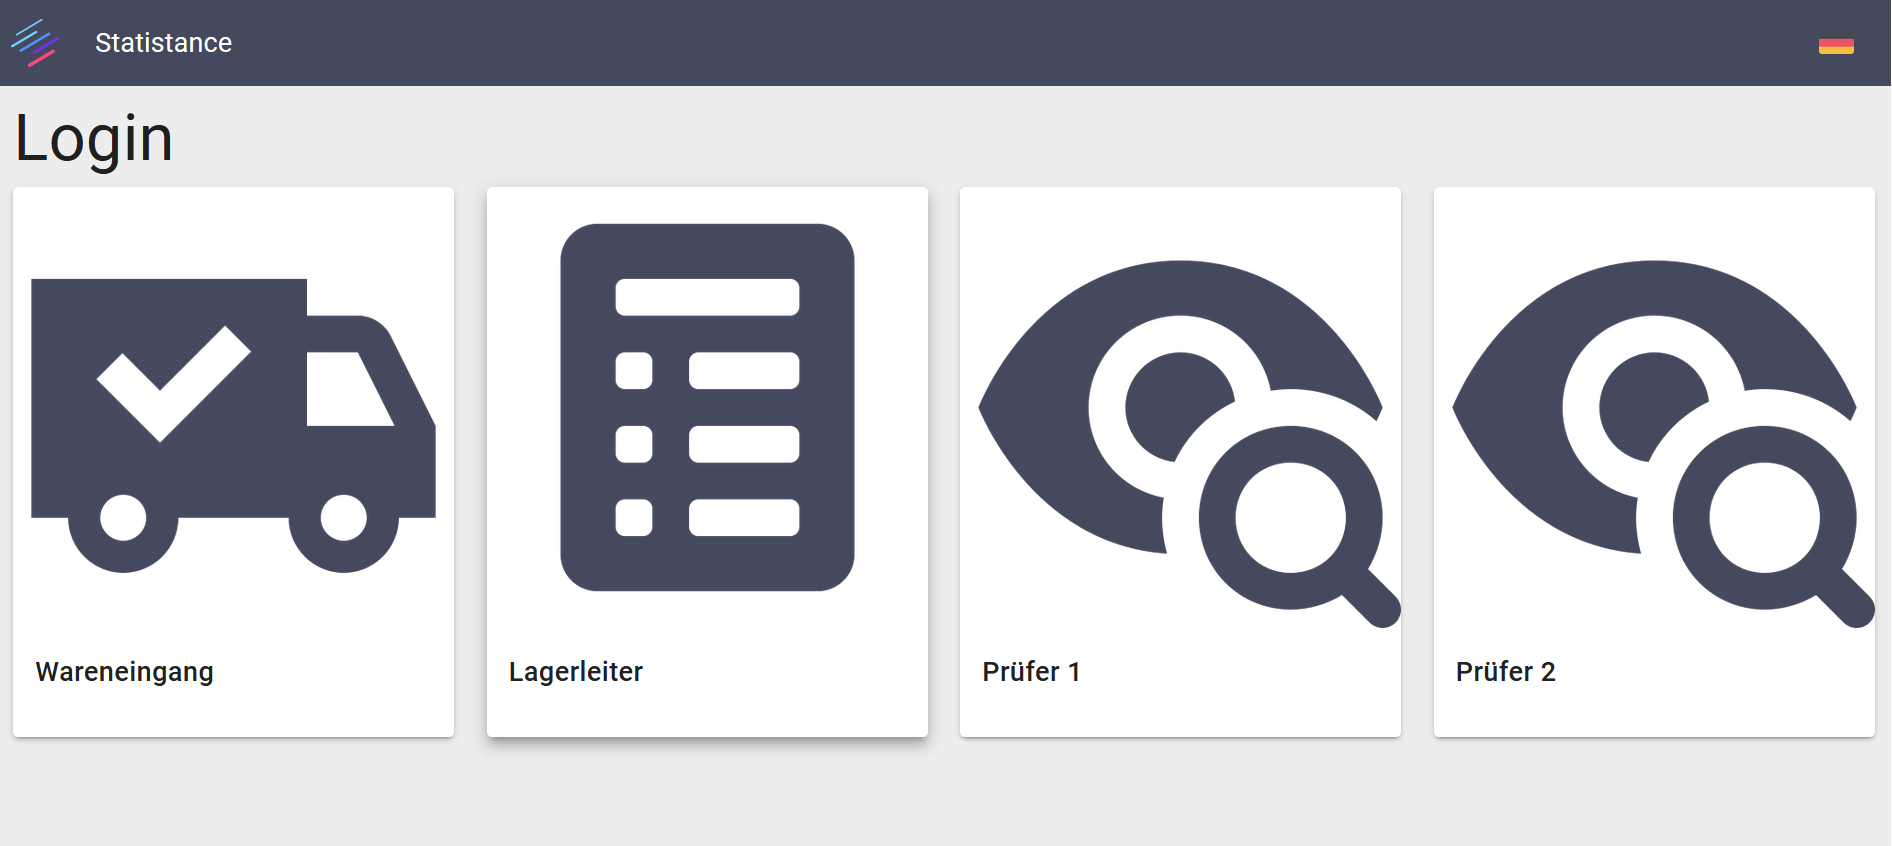
\includegraphics[width=15cm]{images/01_introduction/Statistance_StartPage.PNG}
\caption{Ansichten}
\label{fig:Startpage}
\end{figure}
Eine der Ansichten ist der Wareneingang. Dieser könnte wie in Abbildung \ref{fig:Wareneingang} aussehen. \cite{statistanceWareneingang} Abgeschlossene Lieferungen mit den entsprechenden Informationen, wie Produkte und Losumfang sowie zugewiesene Prüfer und der Fortschritt der Prüfung werden angezeigt. Auch Informationen zum Lieferanten, dem Lieferdatum sowie zum Mitarbeiter, welcher die Lieferung angenommen hat werden abgebildet.
\begin{figure}[!h]
\centering
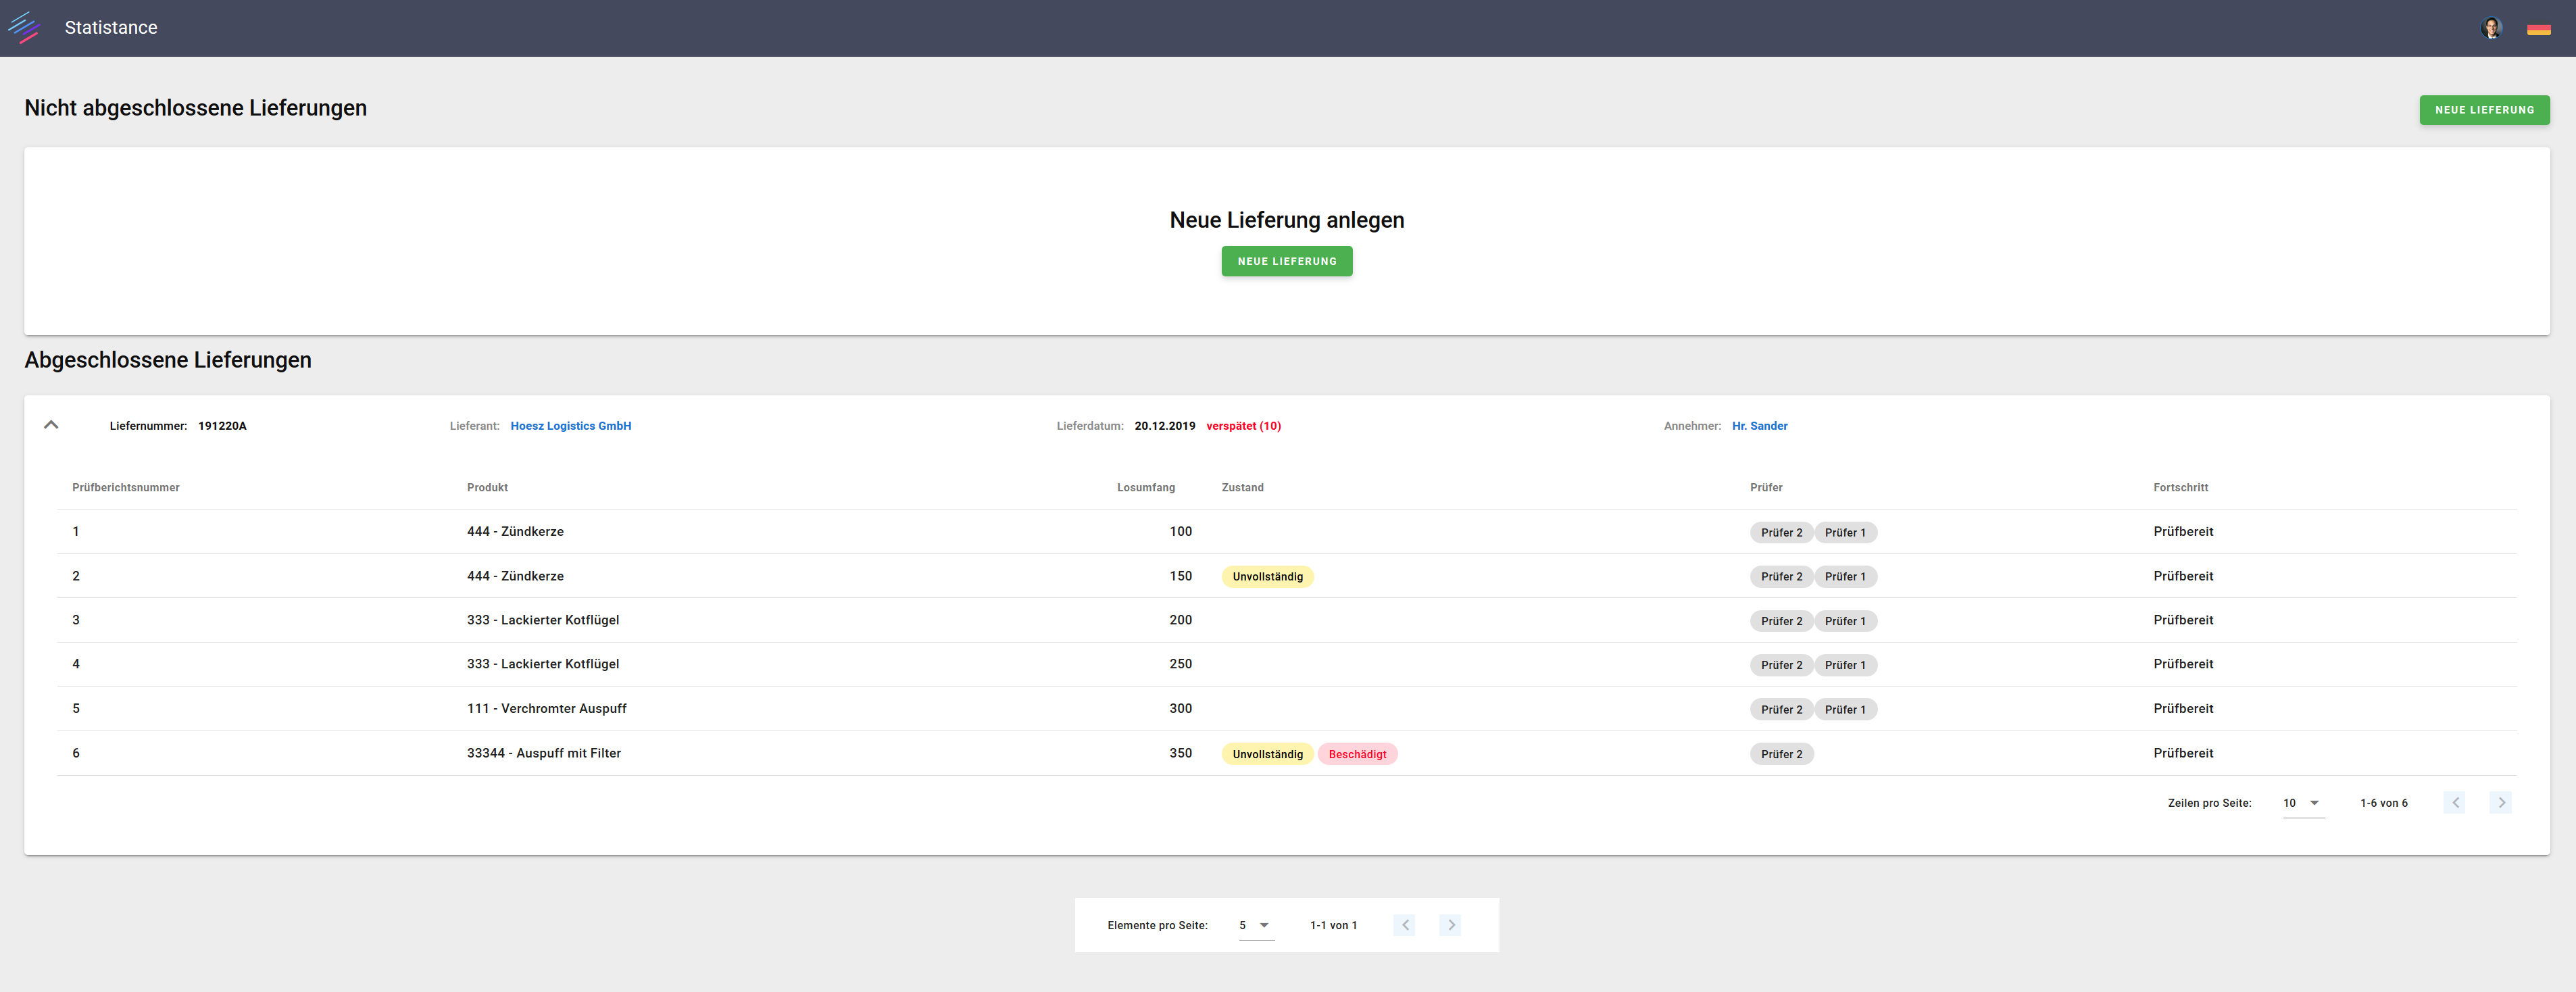
\includegraphics[width=15cm]{images/01_introduction/Statistance_Wareneingang.PNG}
\caption{Beispielhafte Ansicht des Wareneingangs eines Kunden}
\label{fig:Wareneingang}
\end{figure}


Statistance benötigt zur Bereitstellung des auf ERP-System-Daten basierenden Frontends und die statistischen Analysen, die Daten aus dem ERP-System des Kunden. Es werden Informationen zu Lieferanten, Bestellungen, Lieferungen, Produkten, Herstellern und Mitarbeitern für die weitere Verarbeitung benötigt.
\newpage
\section{Aufgabe und Ziel des Projektes}
Im Rahmen des Praxisprojektes sollen die ERP-System-Daten der Kunden aus einer externen Quelle (Warenwirtschafts- und ERP-System) standardisiert in die Anwendung von Statistance zur weiteren Auswertung integriert werden können.
Die sich daraus ergebene Aufgabe konnte in mehrere Teilaufgaben aufgesplittet werden. Zunächst können verschiedene Kunden verschiedene ERP-Systeme verwenden. Der Pilotkunde von Statistance nutzt Sage 100 auf welches sich im Rahmen des Projektes fokussiert wurde. Hierbei mussten Möglichkeiten zur Anbindung von Sage 100 gefunden werden. Zukünftig sollen auch andere ERP-Systeme wie Microsoft Dynamics Navision oder Oracle angebunden werden können. Aus diesen Gründen muss die entwickelte Lösung erweiterbar und skalierbar sein. Weiter sollten die aktuellen Daten aus der Quelle des Kunden für Statistance abrufbar sein. Sinnvoll erschien hier die Möglichkeit verschiedener Batch-Jobs, welche von Statistance gesteuert werden können. Daten können hierdurch im unterschiedlichen Turnus abgerufen werden und Statistance mit aktuellen Daten weiter arbeiten. Die sich daraus ergebenen, konkreten Aufgaben sind nachfolgend aufgelistet.
\begin{enumerate}
\item \textbf{Recherche und Auswahl einer geeigneten Technologie}
\item \textbf{Umsetzung} 
\begin{enumerate}
    \item \textbf{API} (Design, Integration, Dokumentation)
    \item \textbf{Integration des ERP-Systems} (Sage 100)
    \item \textbf{Batch-Job} (Scheduling)
    \item \textbf{Security}
    \item \textbf{Config Managament \& API Gateway}
    \item \textbf{Frontend} 
\end{enumerate}
\end{enumerate}

Das Ergebnis des Projektes soll die in \ref{fig:task} dargestellte Lücke zwischen dem Backend von Statistance und dem ERP-System des Kunden schließen.
\begin{figure}[!h]
\centering
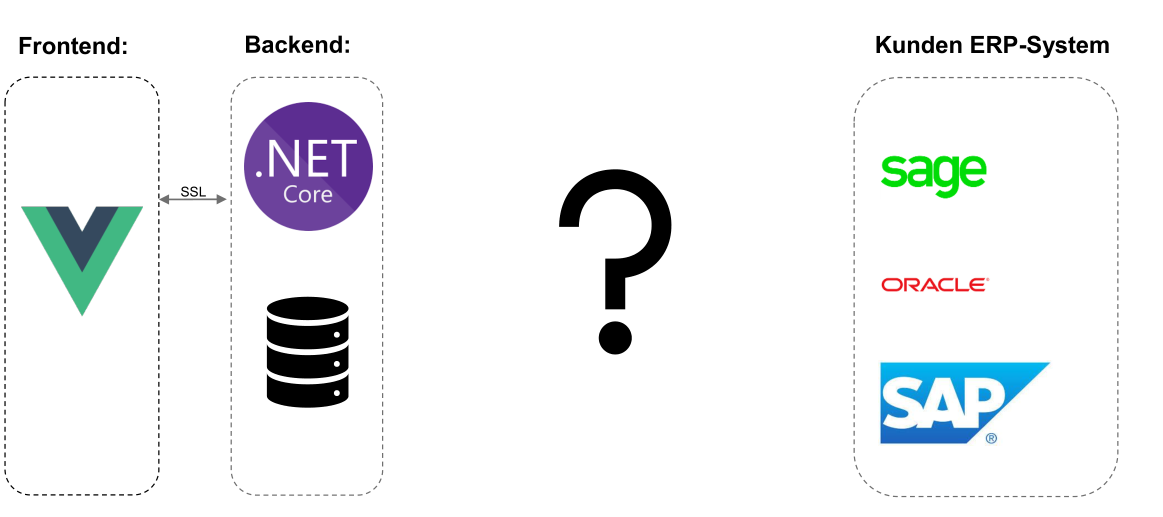
\includegraphics[width=15cm]{images/01_introduction/Aufgabe.PNG}
\caption{Aufgabe}
\label{fig:task}
\end{figure}

